\section{Objetivos globales de competencia}
\begin{itemize}
    \item Los objetivos globales de la planeación estratégica responden a la pregunta \textbf{qué} que queremos lograr estratégicamente en el CP,MP y PL, Para asegurar el logro de la misión y visión de la empresa, ejecutando la EGC. 
        \begin{itemize}
            \item Los objetivos se redactan en infinitivo. Verbos que terminan en ar,er,ir 
            \item Área de enfoque 
            \item Brecha / indicadores X-Y 
            \item Fecha de cumplimiento, \pregunta{Cuándo}, tiene que ser específica. 
        \end{itemize}    
\end{itemize}


%%%%%%%%%%%%%%%%%%%%%%%%%%%%%%%%%%%%%%%%%%%%%%%%%%%%%%%%%%%%%%%%%%%%%%%%%%%%%%%%%%%%%%%%%%
\section{Áreas clave}
\begin{itemize}
    \item Las pareas clave de la organización son los departamentos, funciones, procesos, sistemas, procedimientos de las cuales depende el éxito a fracaso de la organización. 
    \item Construyen las áreas medulares sin las cuáles la organización no podría funcionar y por lo tanto consolidar su misión y visión. 
    \item Son áreas en las cuales se ejecuta la EGC y se toman las decisiones a la luz de los valores de la organización.
    \item La ejecución dentro de las áreas clave se mde por el logro de los OGC. 
    \item Estas áreas NUNCA se dan en outsourcing ya que al depender de ellas el éxito de la organización es necesario tener pleno control de la estrategia y ejecución en las mismas.
    \item Son las áreas que llevan la prioridad de asignación de presupuesto y controlen la ejecución del mismo. 
    \item Se dividen en dos grupos CORE (corazón) y SOPORTE (plataforma que hace el las CORE funcionen).
\end{itemize}
\begin{center}
   \begin{figure}
       \centering
       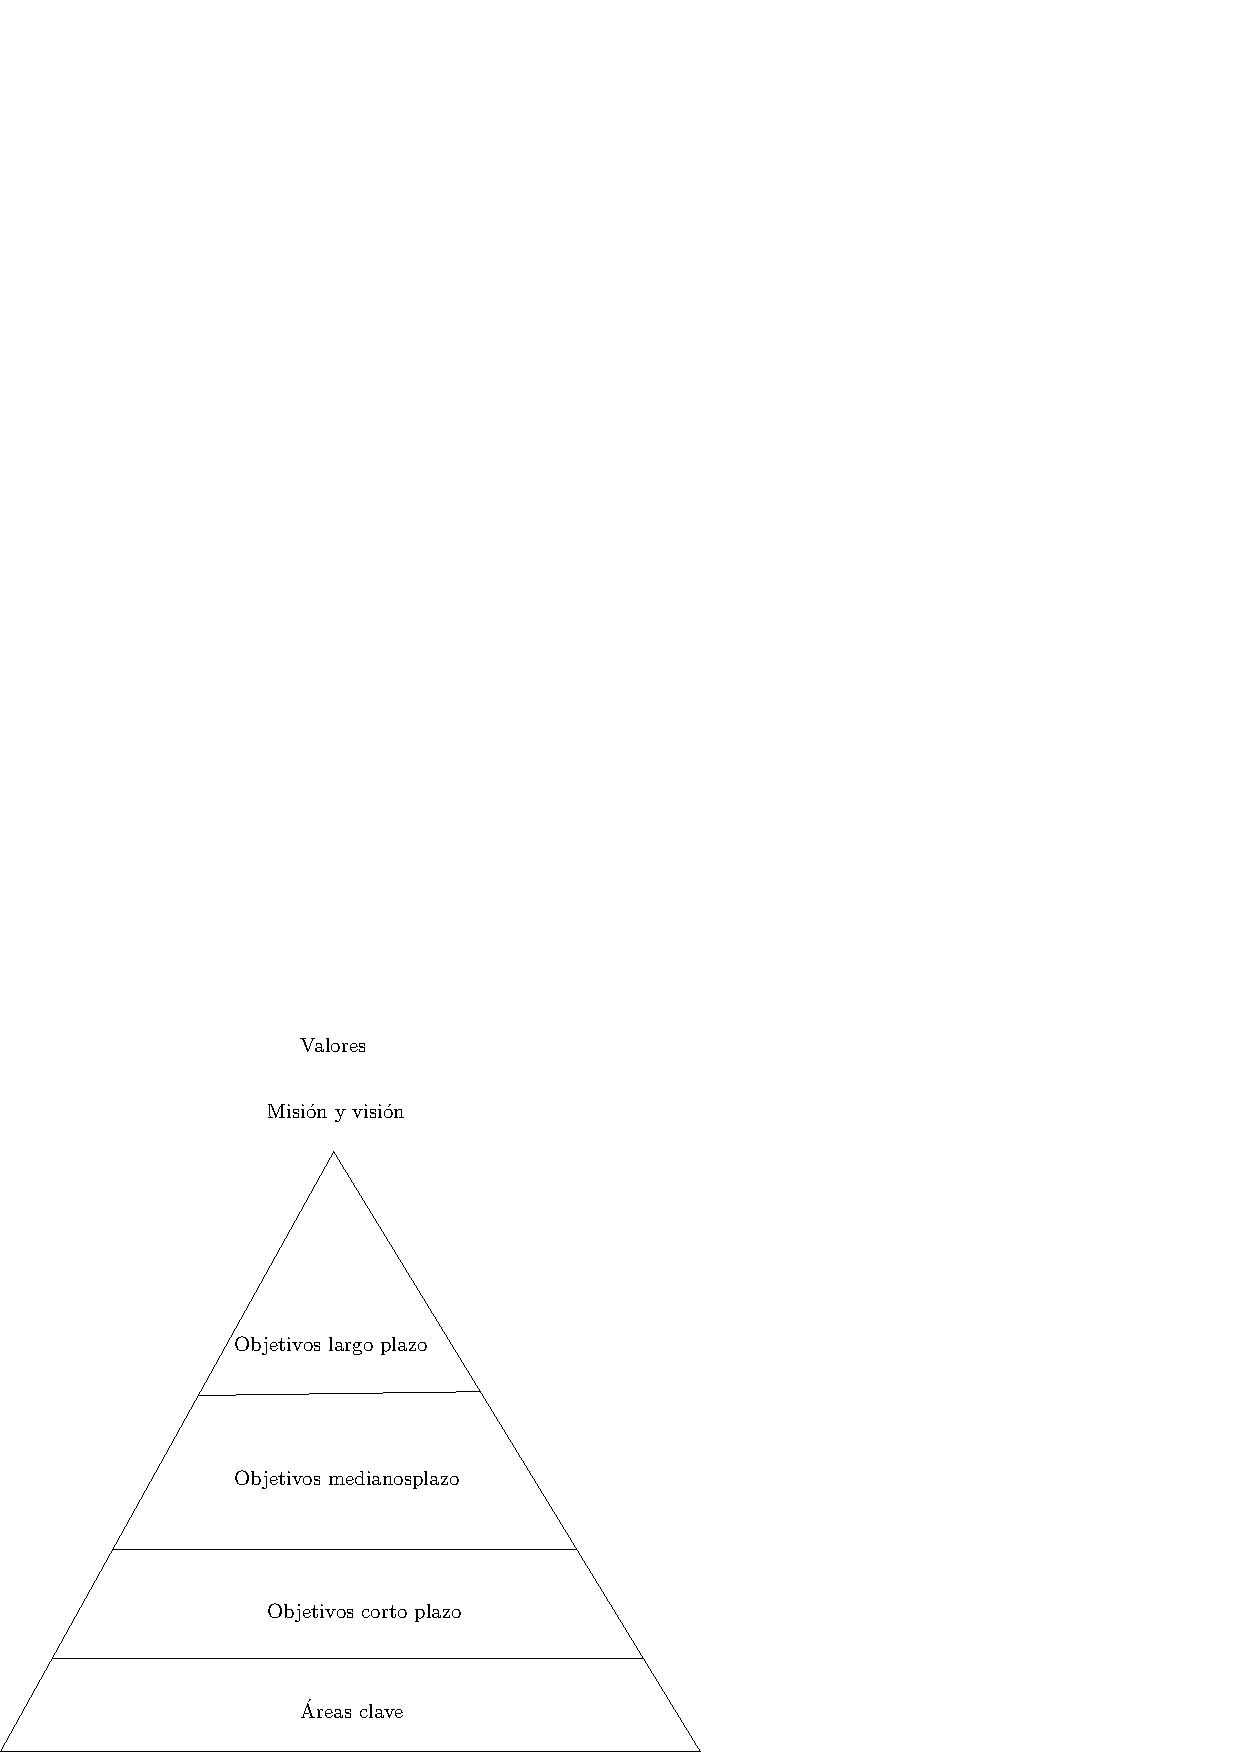
\includegraphics[width=10cm]{./Clases/figs/01}
   \end{figure}
\end{center}
